%Beamer class
\documentclass{beamer}

\usepackage[czech]{babel}
\usepackage[cp1250]{inputenc}
\usepackage{fontenc}
\usepackage{tgheros}
\usepackage{array}
\usepackage{color}
\usepackage{hyperref}

\usetheme{Antibes}
\usecolortheme{crane}


\title[BE1M13VES]{BE1M13VES}
\subtitle[Manufacturing of Electrical Components] {Manufacturing of Electrical Components}
\author[Brejcha]{Michal Brejcha}
\institute[CTU]{CTU in Prague}
\date[Prague, 2017]{Prague, 2017}

\begin{document}
%------------------------------------------------------------------------------
%Uvodni slajd
%------------------------------------------------------------------------------
\frame{\titlepage}

\begin{frame}
\frametitle{Overview} 
\tableofcontents
\end{frame}

\AtBeginSection[]
{
  \begin{frame}
    \frametitle{TOPIC}
    \tableofcontents[currentsection]
  \end{frame}
}

%------------------------------------------------------------------------------
%Base Material Manufacturing
%------------------------------------------------------------------------------
\section{\texorpdfstring{Base Material Manufacturing}{Base Material Manufacturing}}
%------------------------------------------------------------------------------
	\begin{frame}
    \frametitle{Printed Circuit Board}
		Circuit interconnections created as traces of conductor on dielectric substrate.\\

		\begin{center}
			\begin{tabular}{p{0.2\linewidth} p{0.7\linewidth}}
			Conductor: & Cu Film. Thickness is measured in ounces (oz). 1~oz$\approx$35~$\mu$m, most common thickness are 0.5~oz, 1~oz and 2~oz.\\
			Dielectric: & Glass Fabric $+$ Resin. There are several substrates depending on glass to resin volume ratio in the market. Typical parameters are:
			
			\begin{itemize}
				\item $\epsilon_r\approx 3.8 - 5$,
				\item $E_{max}\approx 50$~kV/m,
			\end{itemize}
			\end{tabular}
		\end{center}
	\end{frame}
%------------------------------------------------------------------------------
	\begin{frame}
    \frametitle{Dielectric Glass-Resin Composite - Laminate}
		\small
		\begin{center}
			\begin{tabular}{m{0.4\linewidth} m{0.5\linewidth}}
			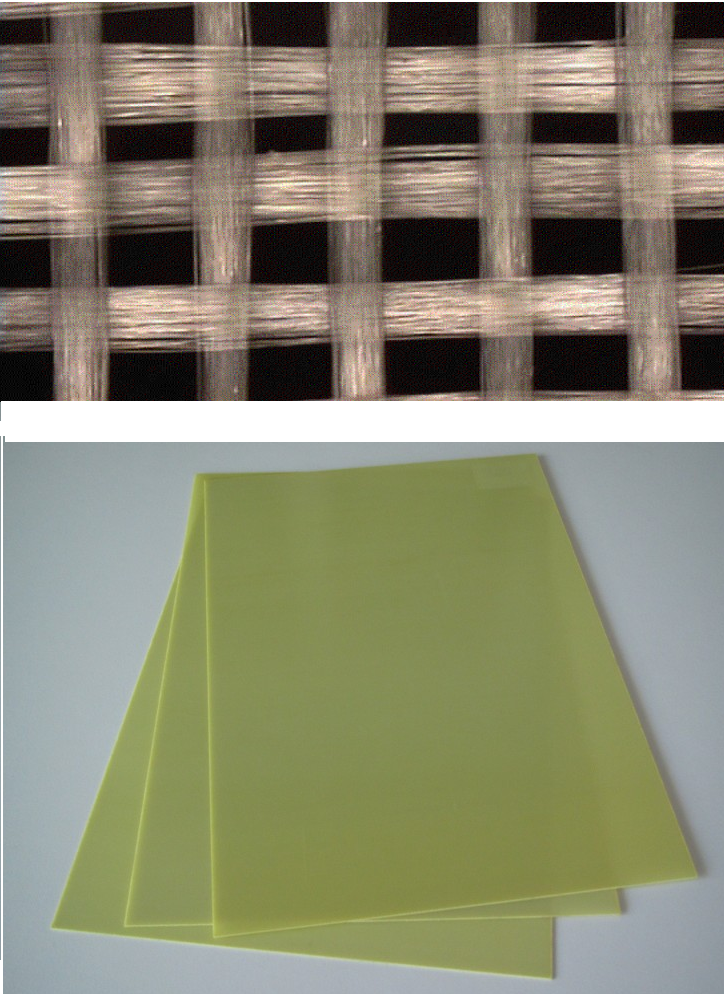
\includegraphics[scale=0.2]{obr23_FR4.png} &
			
			\begin{itemize}
				\item Properties are affected by resin (FR2 phenolic$+$paper, FR4 epoxy$+$glass ) material and warp and fill of the glass,
				\item common thickness of the layers are from 0.04 mm up to 2 mm.
				\item FR4 are core materials of laminate with cured resin.
				\item Pre-preg - stands for "pre-impregnated", resin is cured to an intermediate stage.
			\end{itemize}
			\end{tabular}
		\end{center}
	\end{frame}
%------------------------------------------------------------------------------
	\begin{frame}
    \frametitle{Lamination process}
		\small
		\begin{center}
			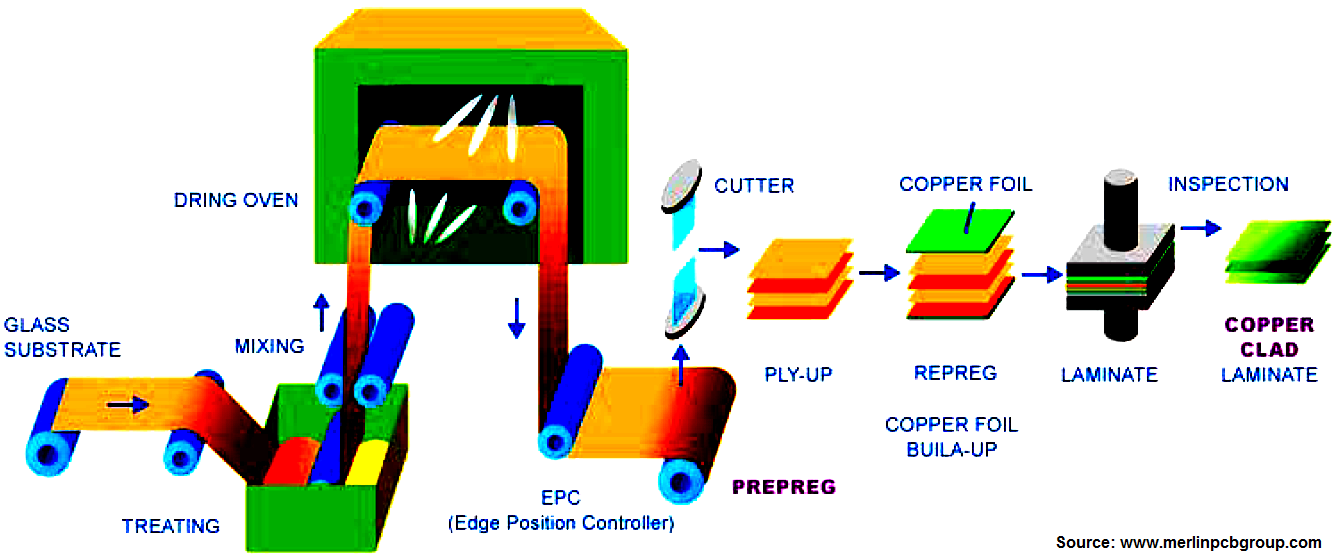
\includegraphics[scale=0.3]{obr28_laminace.png}
		\end{center}
	\end{frame}
%------------------------------------------------------------------------------
	\begin{frame}
    \frametitle{Coper Foil Manufacturing}

		\begin{center}
			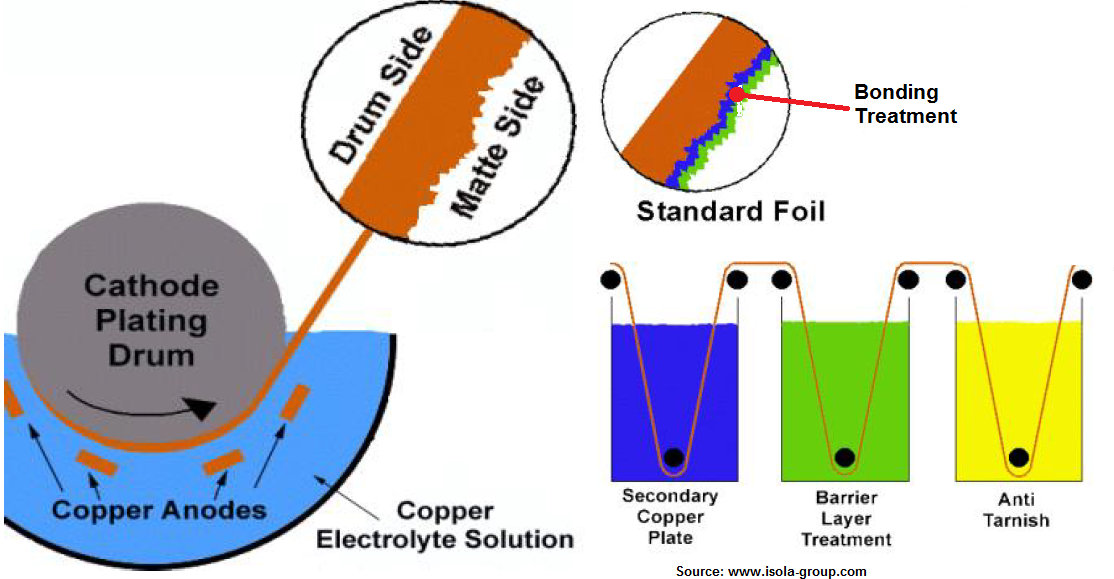
\includegraphics[scale=0.25]{obr24_Cu.png}
		\end{center}
		
		\begin{itemize}
			\item Copper is electroplated onto a rotating drum.
			\item Treatments are applied to: micro-roughen surface for adhesion, plate barrier layer, coat with anti-tarnish
		\end{itemize}
	\end{frame}
%------------------------------------------------------------------------------
	\begin{frame}
    \frametitle{FR4 Core Material}

		\begin{center}
			\begin{tabular}{m{0.4\linewidth} m{0.5\linewidth}}
			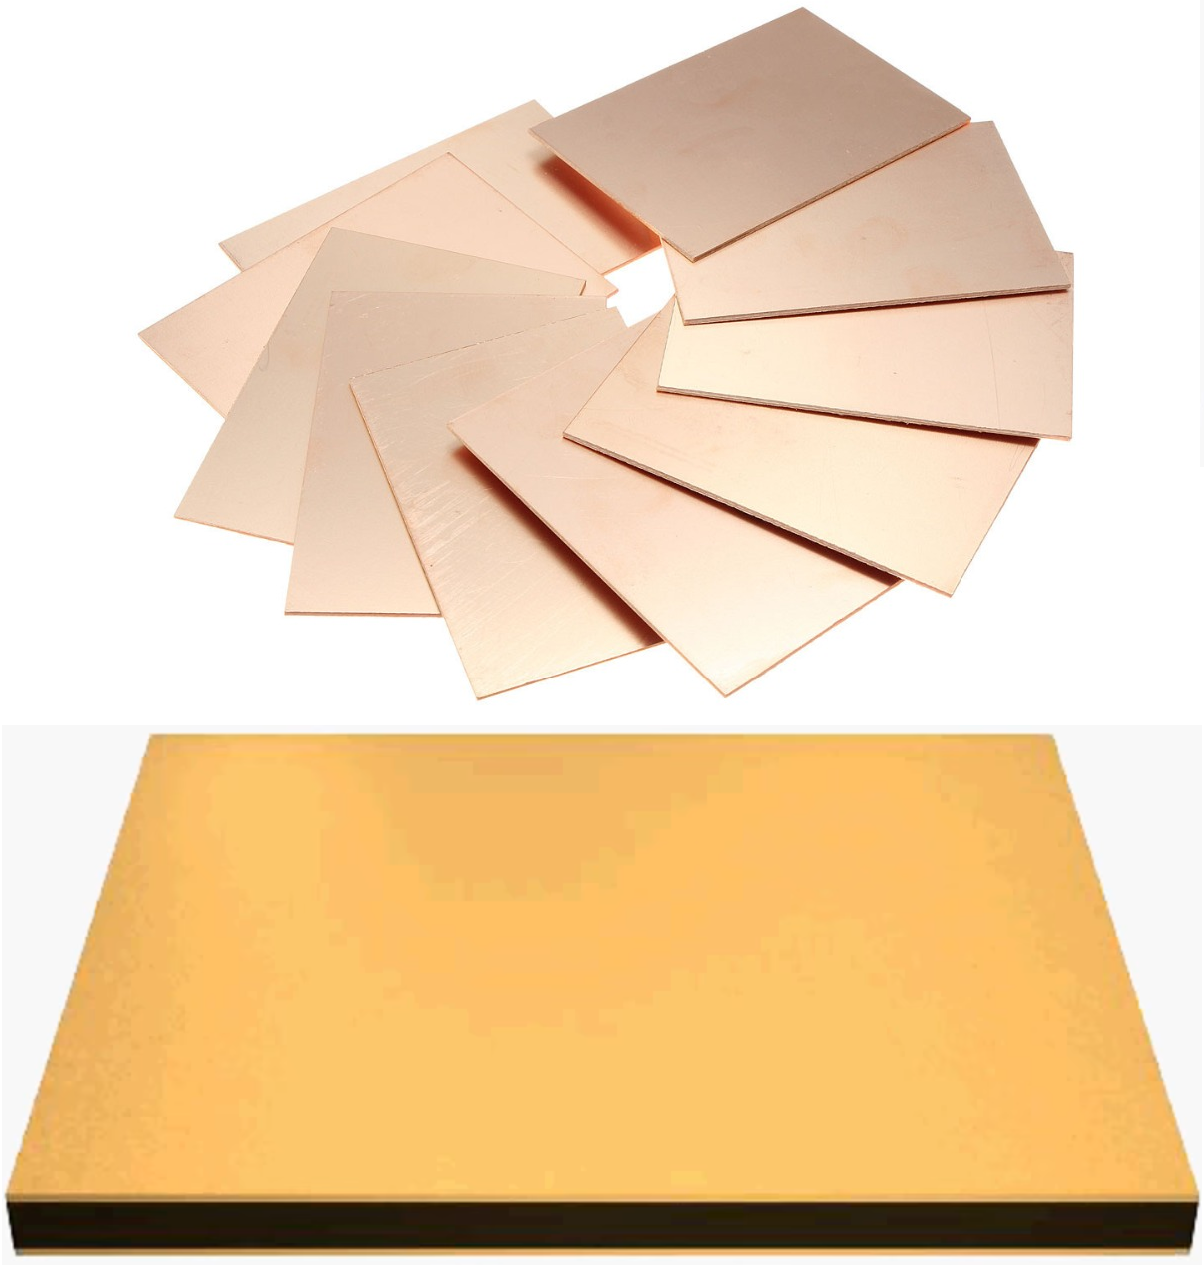
\includegraphics[scale=0.12]{obr02_jadro.png} & \textbf{Lay up}
			\begin{itemize}
				\item Sandwich, FR4 core is between two (can be also one sided) Cu layers,
				\item layers are bonded and resin is cured at specific pressure (from $1.9$~MPa to $2.8$~MPa) and temperature (about 190~$^\circ$F),
			\end{itemize}
			\end{tabular}
		\end{center}
		
		\begin{itemize}
			\item this base is used as a core for multilayer PCBs or for one or two sided PCBs.
		\end{itemize}
	\end{frame}
%------------------------------------------------------------------------------
%PCB Manufacturing
%------------------------------------------------------------------------------
\section{\texorpdfstring{PCB Manufacturing}{PCB Manufacturing}}
%------------------------------------------------------------------------------
	\begin{frame}
    \frametitle{Drilling the holes to the core}

		\begin{center}
			\begin{tabular}{m{0.5\linewidth} m{0.4\linewidth}}
			\textbf{This is done only if:}
			\begin{itemize}
				\item it is one or two sided pcb or
				\item there are some vias only in the inner layers.
			\end{itemize}
			 & 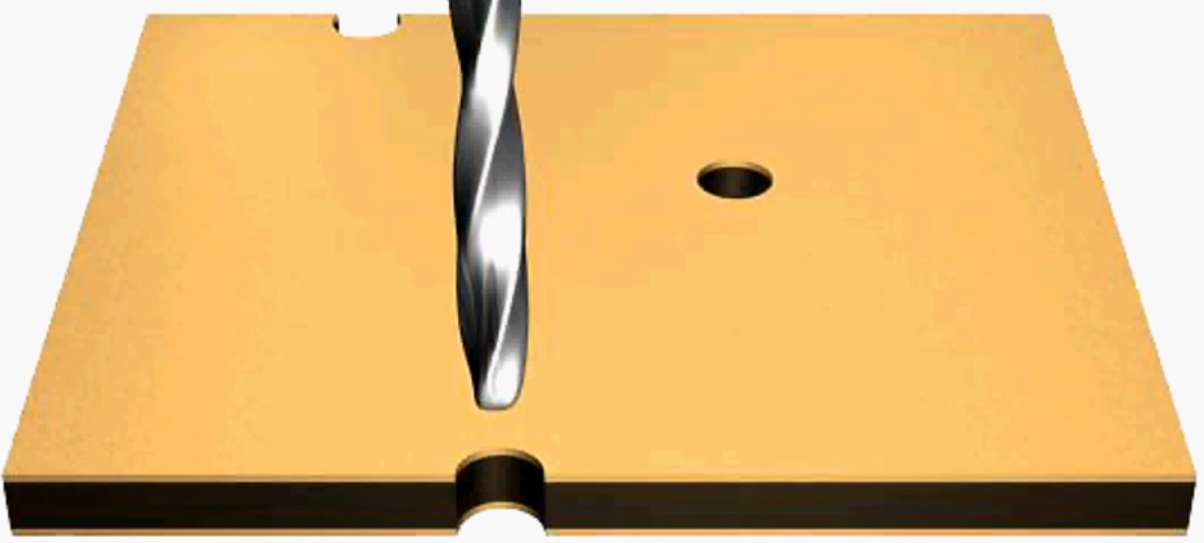
\includegraphics[scale=0.12]{obr03_jadroVrtani.png}
			\end{tabular}
		\end{center}
		The connection between sides is ensured after through hole plating.
		\begin{center}
		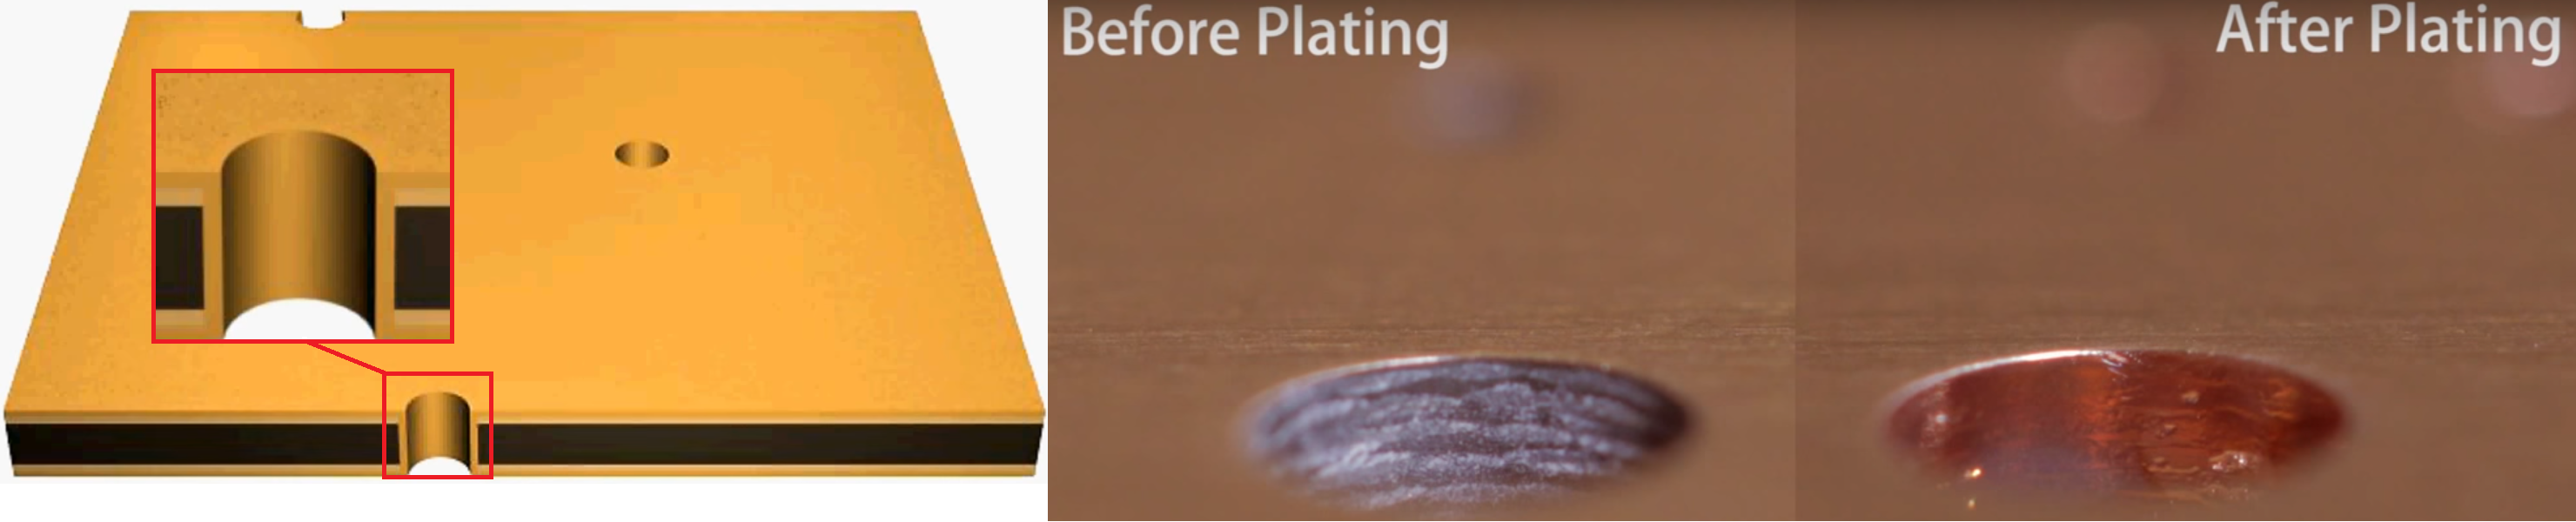
\includegraphics[scale=0.14]{obr04_jadroProkovy.png}
		\end{center}
	\end{frame}
%------------------------------------------------------------------------------
	\begin{frame}
    \frametitle{Photo-resist deposition}

		\begin{flushleft}
			\begin{tabular}{m{0.5\linewidth} m{0.4\linewidth}}
			\begin{itemize}
				\item resist is applied by heat and pressure to the metal surfaces of the core,
				\item it is rolled out in most of the cases,
				\item it can be also sprayed in case of piece production (amateurs),
				\item the film is sensitive to UV light,
			\end{itemize}
			 & 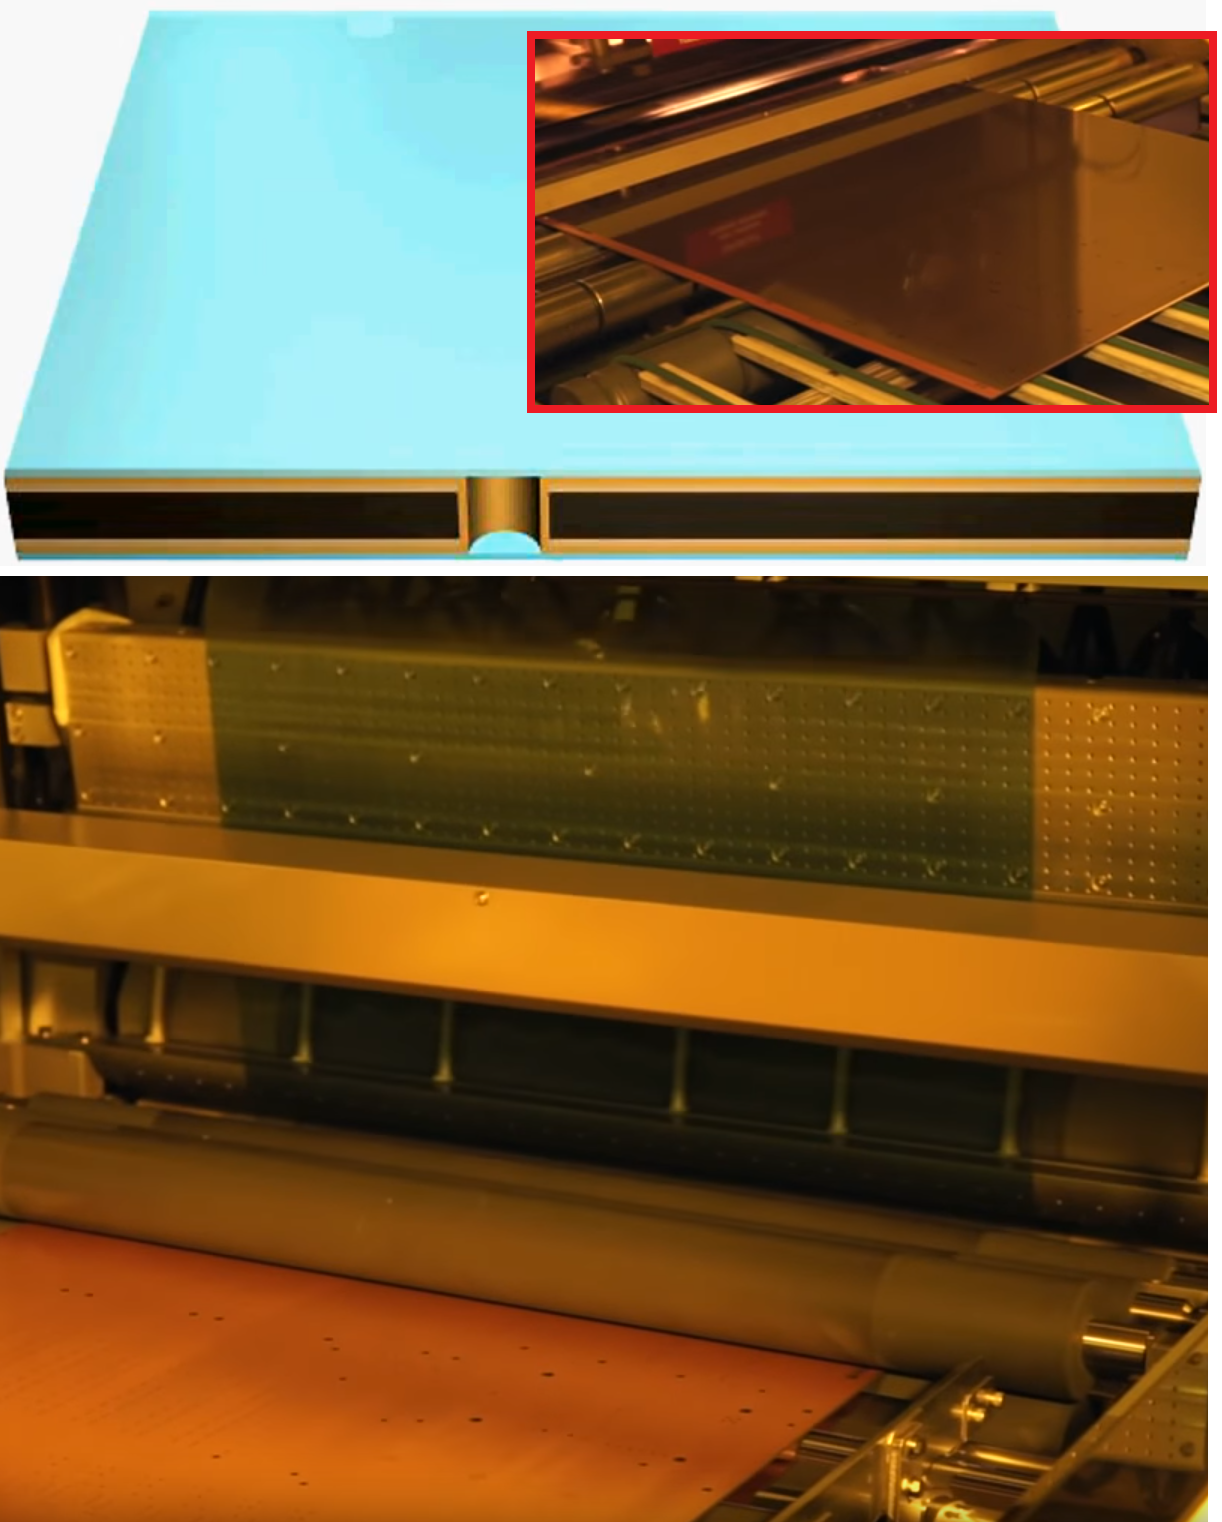
\includegraphics[scale=0.12]{obr05_jadroFotofilm.png}
			\end{tabular}
			\begin{tabular}{m{0.9\linewidth}}
			\begin{itemize}
				\item yellow light is used in most image processing areas to prevent inadvertent exposure of the resist.
			\end{itemize}
			\end{tabular}
		\end{flushleft}

	\end{frame}
%------------------------------------------------------------------------------
	\begin{frame}
    \frametitle{Basic Types of resists}

		\begin{center}
			\begin{tabular}{m{0.35\linewidth} m{0.55\linewidth}}
			 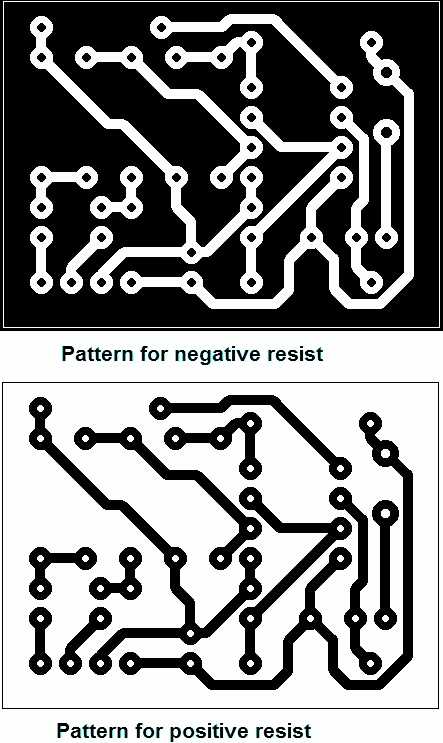
\includegraphics[scale=0.9]{obr27_negativAPozitiv.png} &
				There are two possible reaction of the resist:
				
				\begin{enumerate}
					\item illuminated parts are polymerized (hardened) or
					\item they are chemical changed and then soluble in developer.
				\end{enumerate}
				First type is called negative resist, because the negative pattern (mask) is needed. Second one is positive resist. The negative resist is more common in mass production.
			\end{tabular}
		\end{center}
		
	\end{frame}
%------------------------------------------------------------------------------
	\begin{frame}
    \frametitle{Exposition and developing}

		\begin{center}
			\begin{tabular}{m{0.35\linewidth} m{0.55\linewidth}}
			 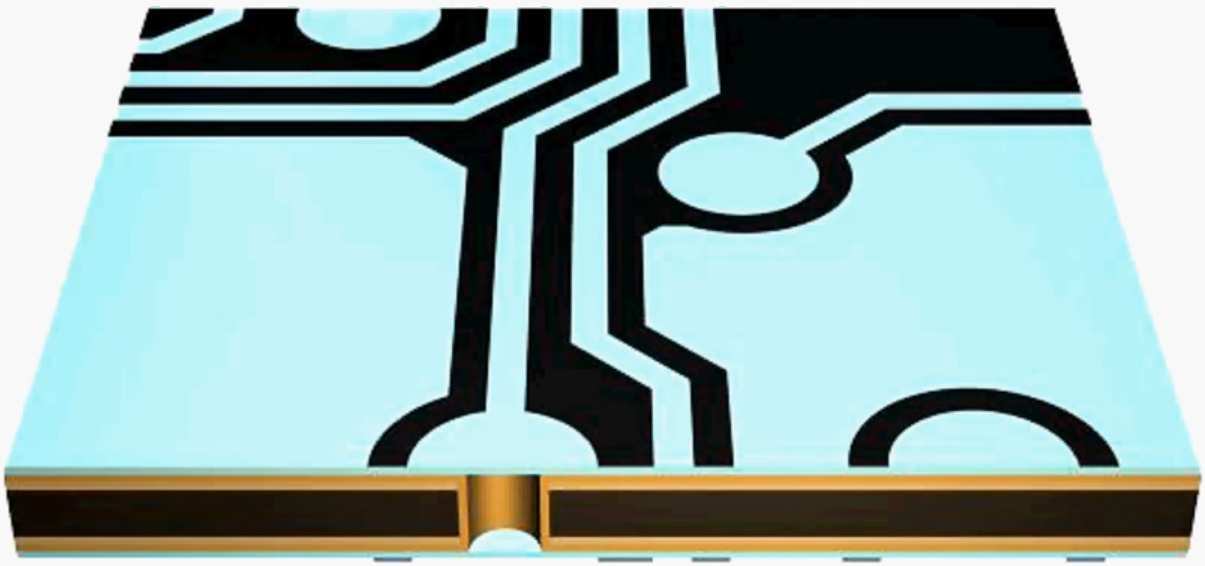
\includegraphics[scale=0.12]{obr06_jadroOsvit.png} &
				
				\begin{itemize}
					\item[$\Leftarrow$] The exposition is made by UV light,
					\item[$\Downarrow$] after that the unwanted resist is washed (developed) and only the pattern stays on the board.
				\end{itemize}
			\end{tabular}
			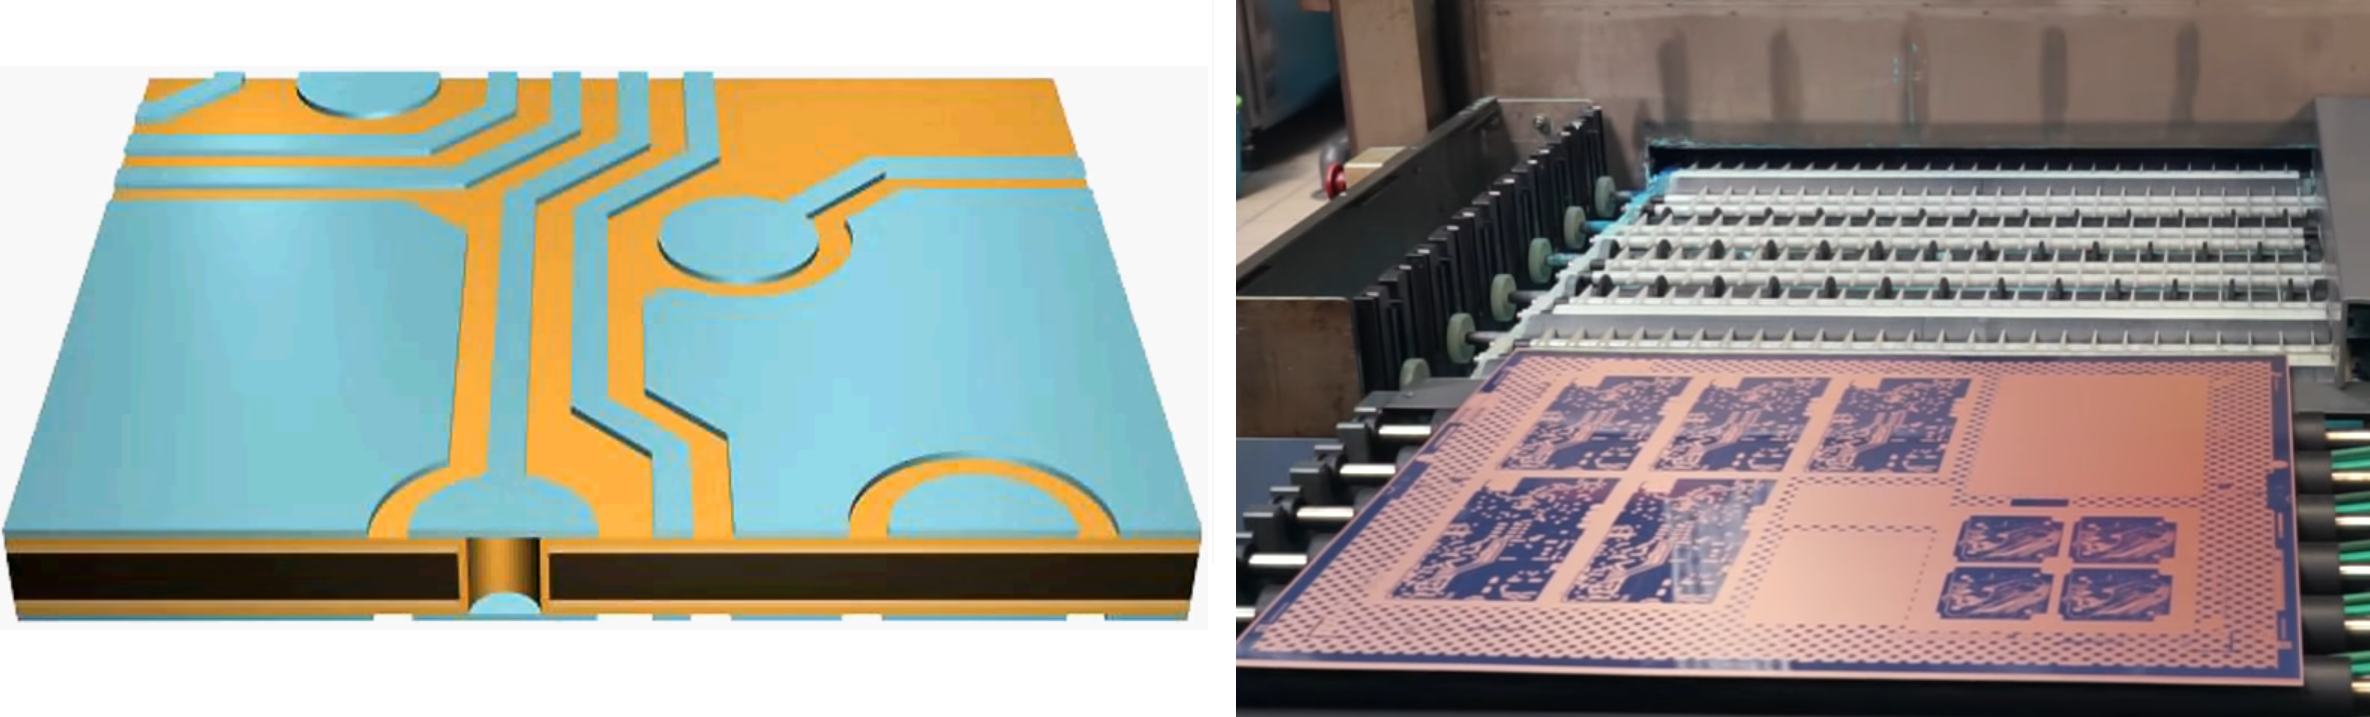
\includegraphics[scale=0.15]{obr07_jadroVyvolani.png}
		\end{center}
		
	\end{frame}
%------------------------------------------------------------------------------
	\begin{frame}
    \frametitle{Etching}

		\begin{center}
			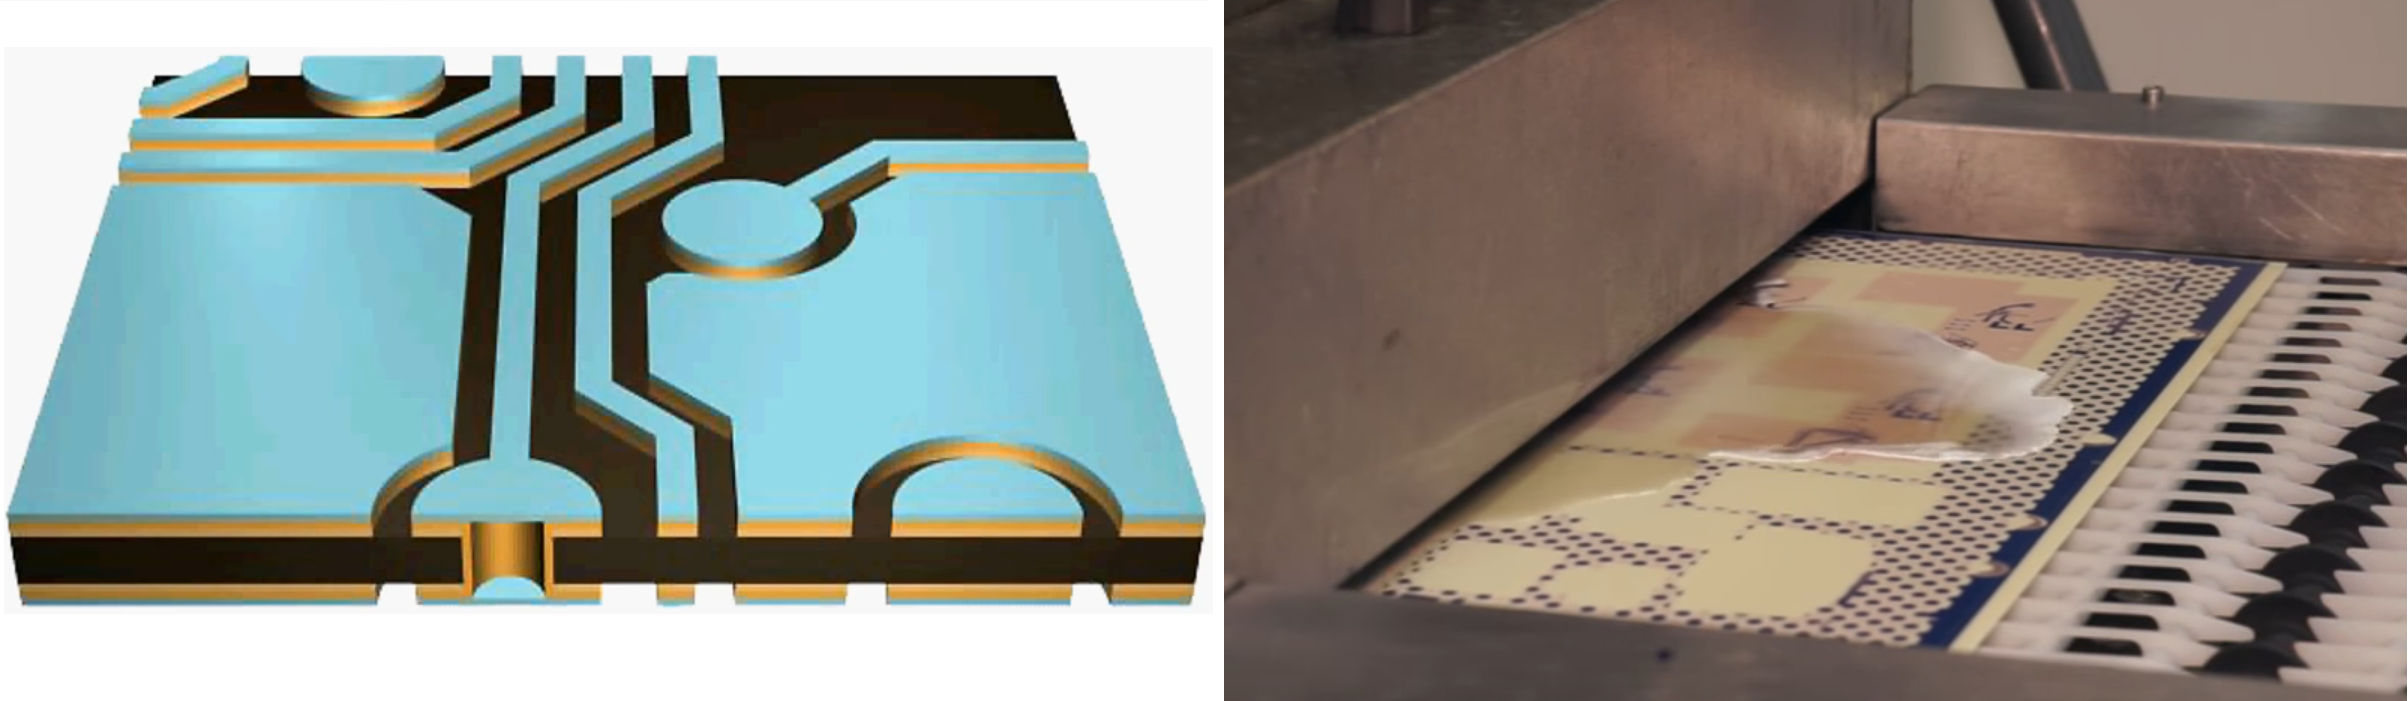
\includegraphics[scale=0.15]{obr08_jadroLeptani.png}
		\end{center}
		
		\begin{itemize}
			\item If there are plated holes, then they must be covered by the resist.
			\item The unwanted copper is solute in an acid.
			\item Etching liquid are mainly copper chloride solution, ferric chloride liquid, alkaline etching, acid/hydrogen peroxide (hydrogen peroxide) etching.
		\end{itemize}
	\end{frame}
%------------------------------------------------------------------------------
	\begin{frame}
    \frametitle{Core PCB}

		\begin{center}
			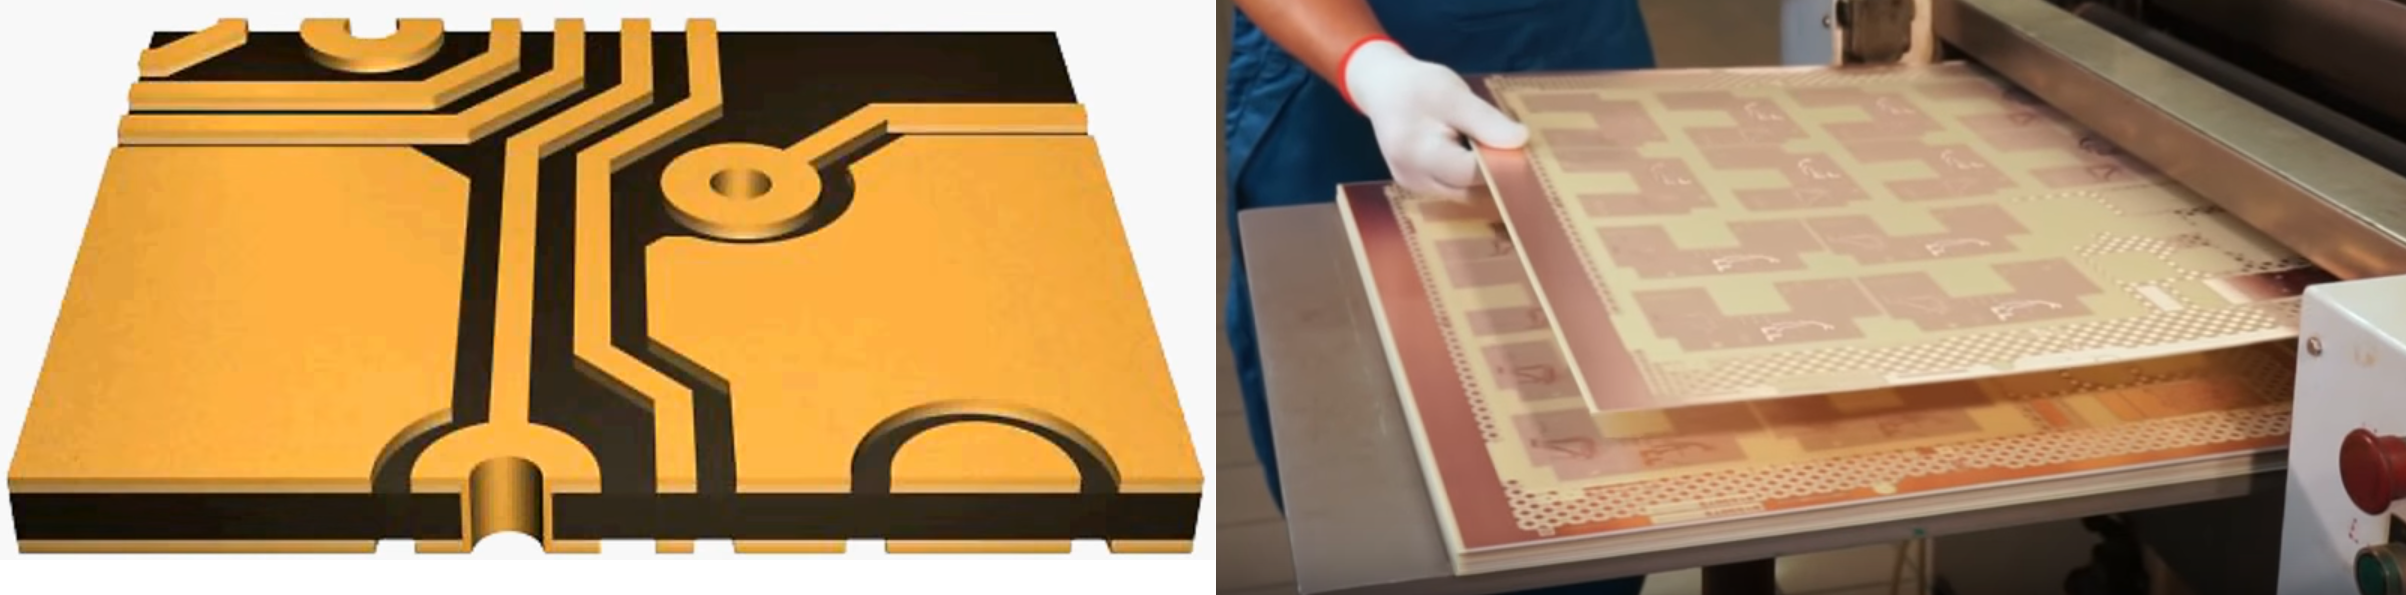
\includegraphics[scale=0.15]{obr09_jadroHotovo.png}
		\end{center}
		
		\begin{itemize}
			\item The core is cleaned from the resist and the pattern is checked via automated optical inspection.
			\item If there are only two track layers then the process continues with solder mask deposition.
			\item In case of multilayer PCB the process continues with lamination of other layers.
		\end{itemize}
	\end{frame}
%------------------------------------------------------------------------------
%PCB Manufacturing
%------------------------------------------------------------------------------
\section{\texorpdfstring{Multilayer PCB Manufacturing}{Multilayer PCB Manufacturing}}
%------------------------------------------------------------------------------
	\begin{frame}
    \frametitle{Adding other Layers}

		\begin{center}
			\includegraphics[scale=0.10]{obr21_Platovani.png}
		\end{center}
		\begin{flushleft}
			\textbf{Hand-made sandwich:}
		\end{flushleft}
		\begin{center}
			\begin{tabular}{p{0.45\linewidth} p{0.45\linewidth}}
			
		  \begin{enumerate}
			  \setcounter{enumi}{0}
			  \item Placing bottom Cu and prepreg layer,
			  \item placing core layer,
		  \end{enumerate}
			&
			\begin{enumerate}
			  \setcounter{enumi}{2}
			  \item placing top prepreg layer,
			  \item placing top Cu layer.
		  \end{enumerate}
			\end{tabular}
		\end{center}
	\end{frame}
%------------------------------------------------------------------------------
	\begin{frame}
    \frametitle{Bonding the Layers by Heat and Preassure}

		\begin{center}
			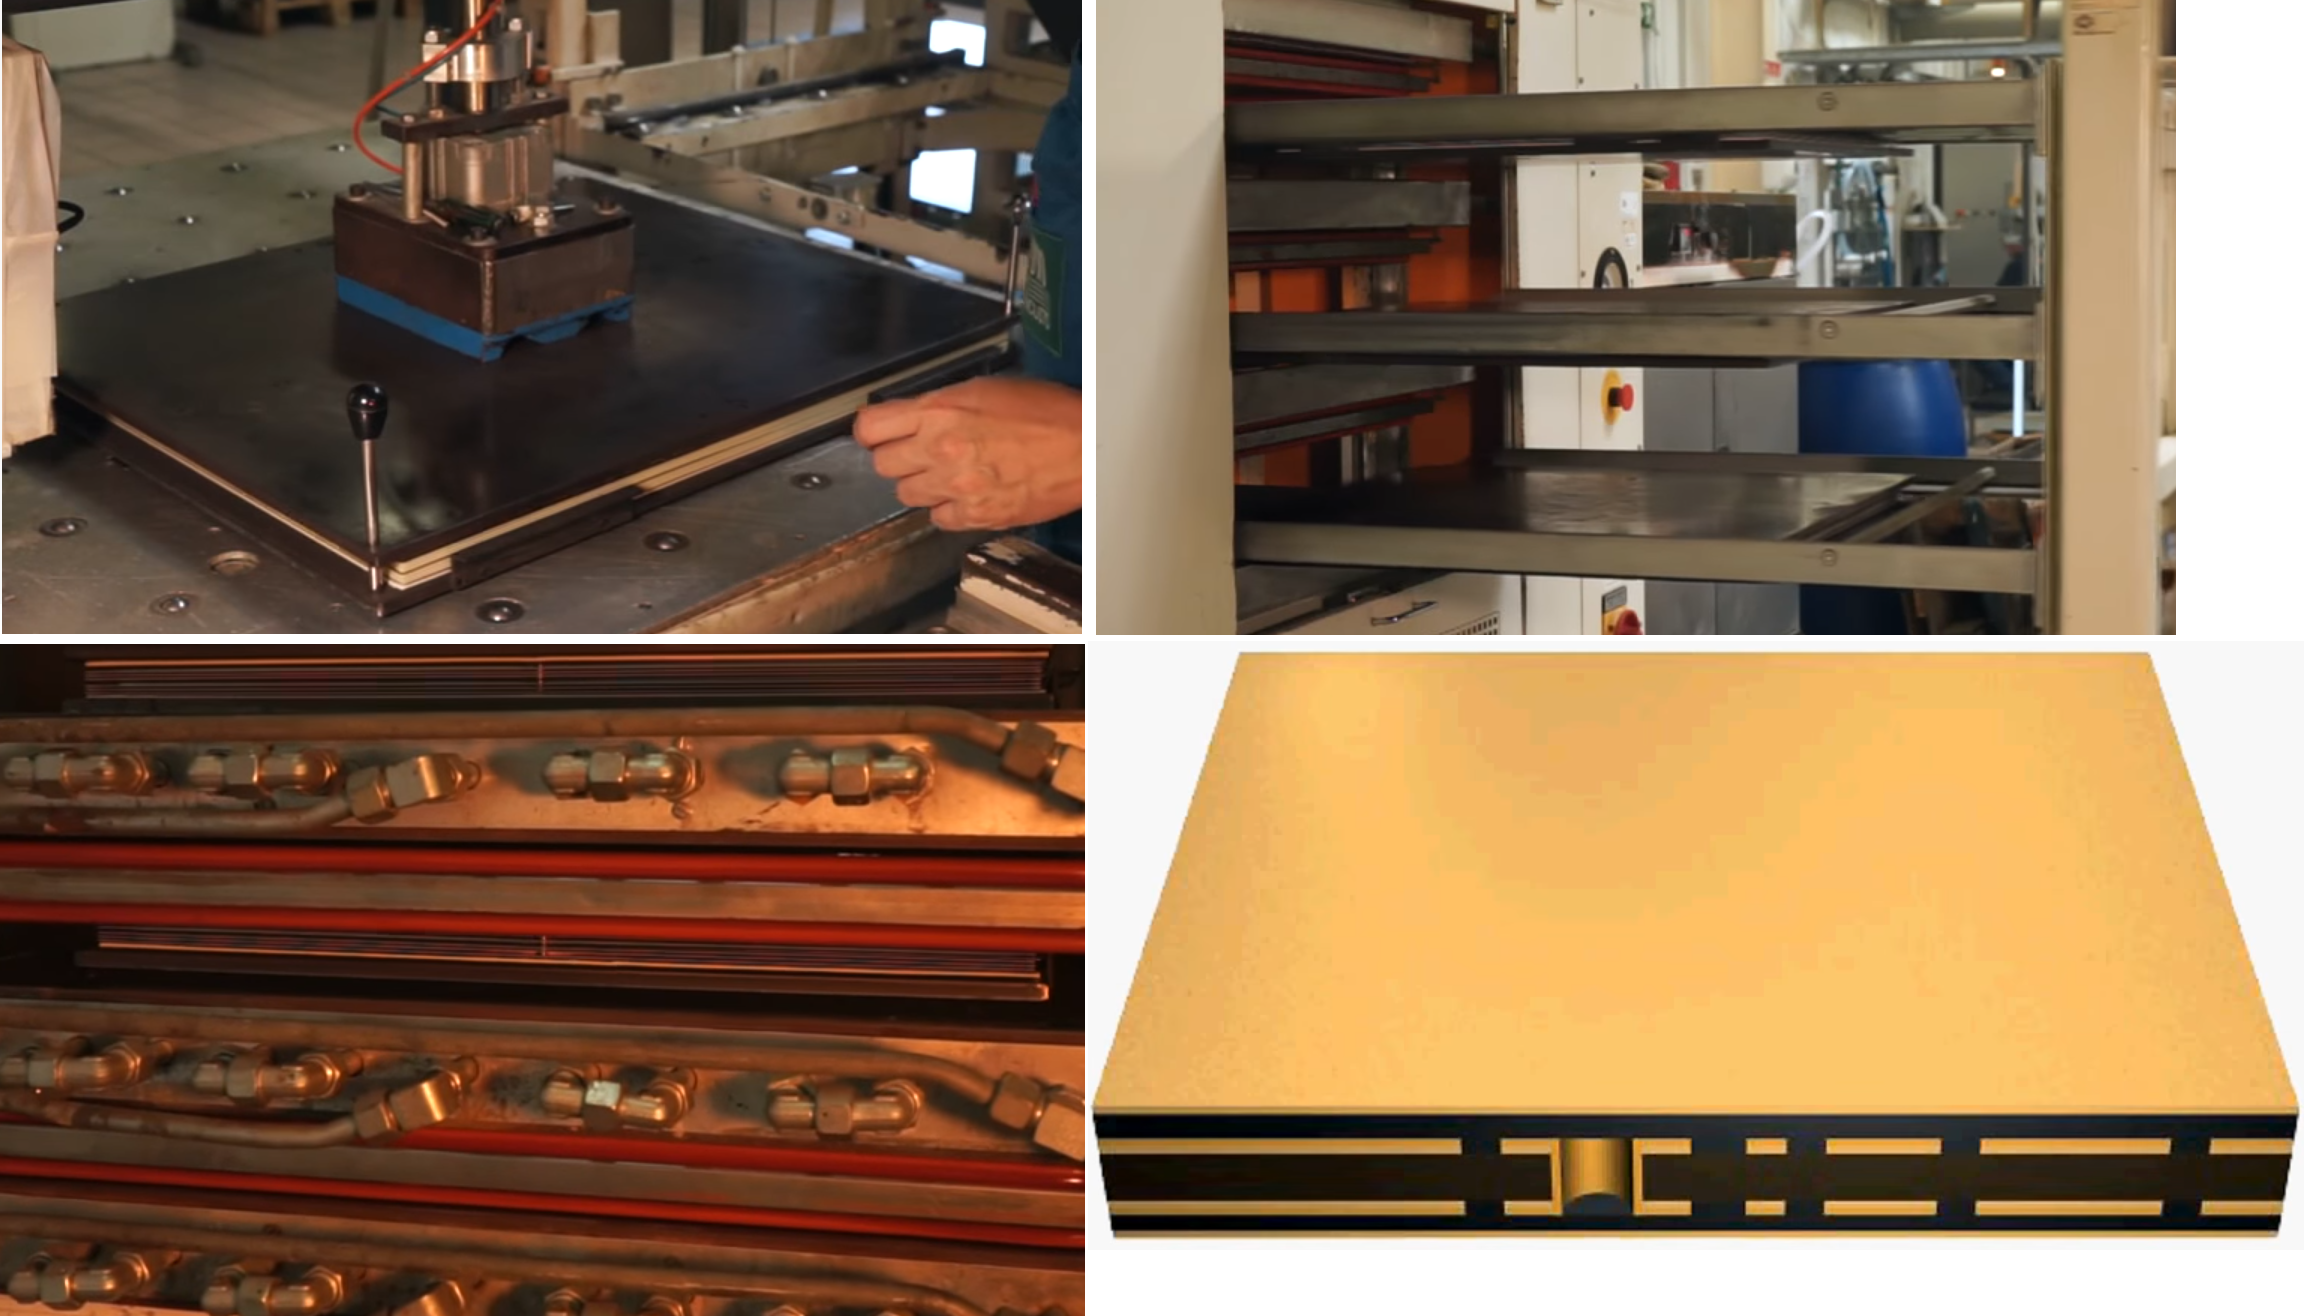
\includegraphics[scale=0.15]{obr11_vnejsiCuFilm.png}
		\end{center}
		
		\begin{itemize}
			\item Use the similar lamination process as in case of core laminate. The resin is cured at about $190$~$^\circ$C.
		\end{itemize}
	\end{frame}
%------------------------------------------------------------------------------
	\begin{frame}
    \frametitle{Drilling}

		\begin{center}
			\begin{tabular}{m{0.45\linewidth} m{0.45\linewidth}}
			 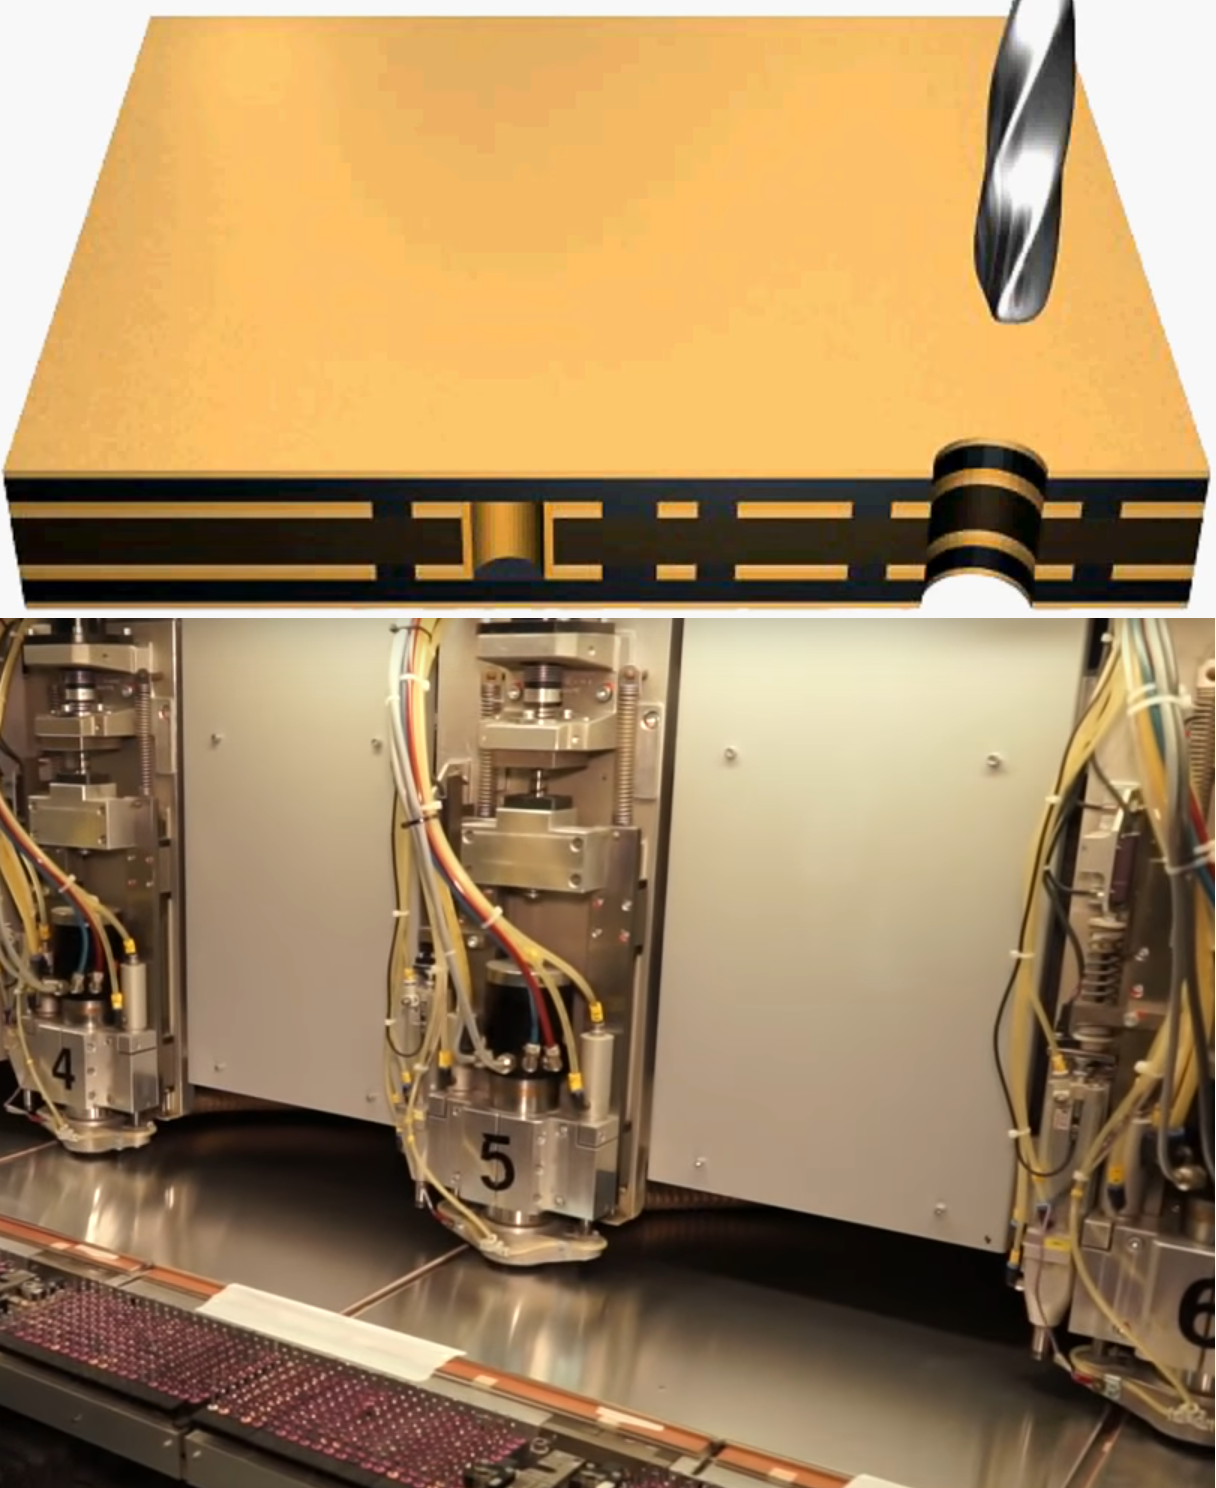
\includegraphics[scale=0.15]{obr12_vnejsiVrtani.png} &
				
				\begin{itemize}
					\item Several PCBs are drilled together at a drill station.
					\item Similary to core manufacturing, the next process is through hole plating.
				\end{itemize}
			\end{tabular}
		\end{center}
	\end{frame}
%------------------------------------------------------------------------------
	\begin{frame}
    \frametitle{Pattern Processing}
		...is the same as in case of the core pattern processing:
		\begin{center}
		
			\begin{tabular}{m{0.05\linewidth} m{0.38\linewidth} m{0.05\linewidth} m{0.38\linewidth}}
			 \Large & 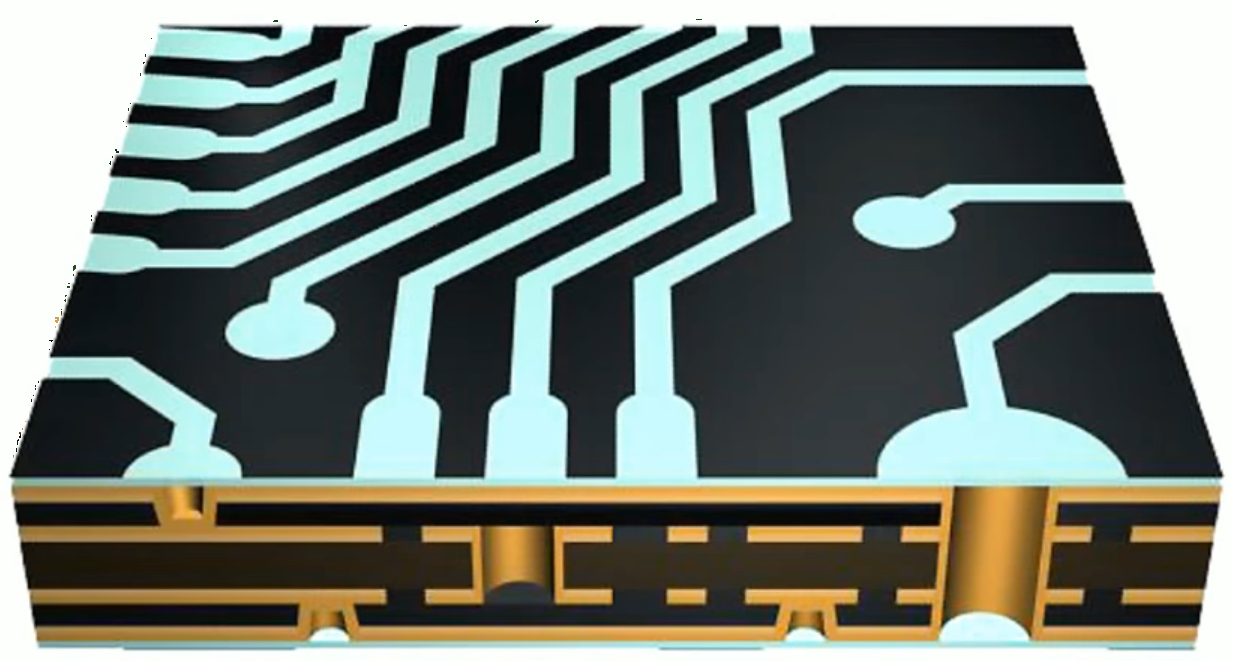
\includegraphics[scale=0.12]{obr13_vnejsiOsvit.png} & \Large\textbf{$\rightarrow$} & 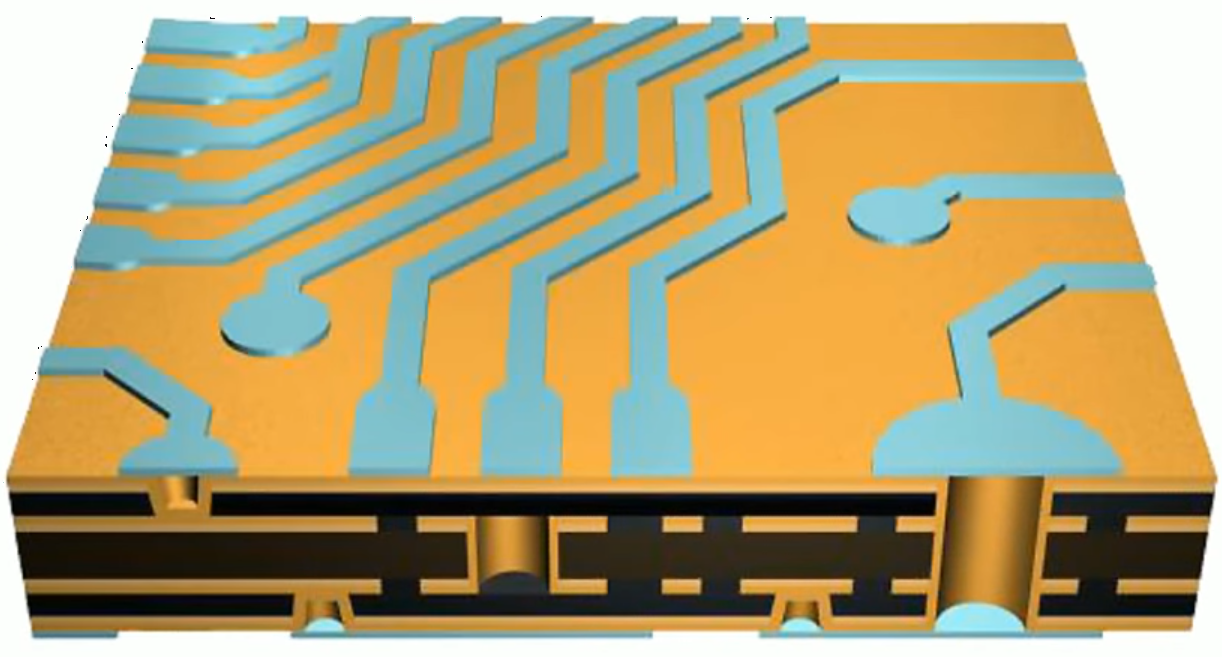
\includegraphics[scale=0.12]{obr14_vnejsiVyvolani.png}\\
			 & Resist deposition and UV illumination & & Developing \\
			 \Large\textbf{$\hookrightarrow$} & 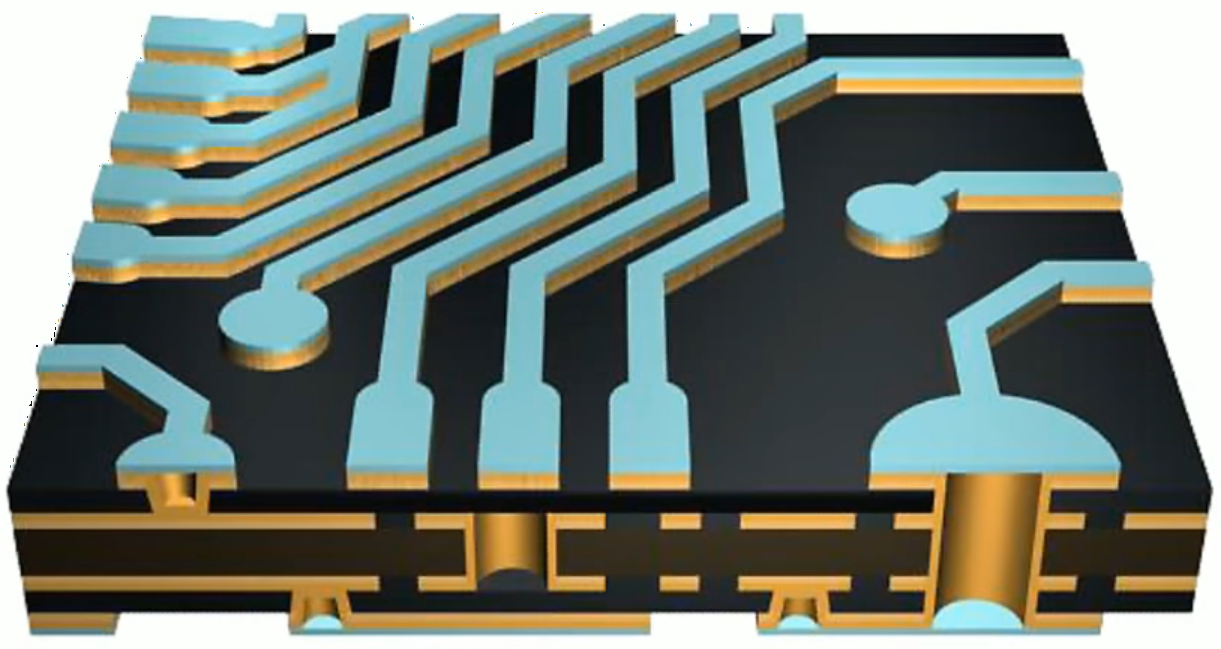
\includegraphics[scale=0.12]{obr15_vnejsiLeptani.png} & \Large\textbf{$\rightarrow$} & 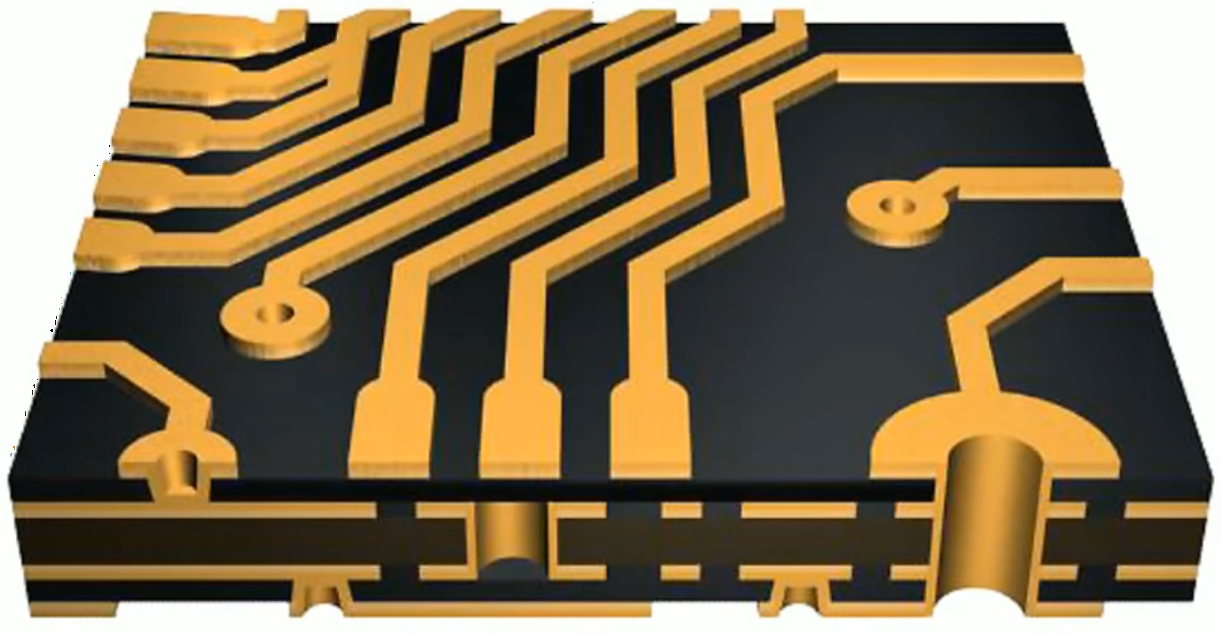
\includegraphics[scale=0.12]{obr16_vnejsiHotovo.png}\\
			& Etching & & Resist cleaning
			\end{tabular}
		\end{center}
	\end{frame}
%------------------------------------------------------------------------------
	\begin{frame}
    \frametitle{Solder-mask Processing}
		...is the same as in case of the core pattern processing:
		\begin{center}
		
			\begin{tabular}{m{0.05\linewidth} m{0.38\linewidth} m{0.05\linewidth} m{0.38\linewidth}}
			 \Large & \includegraphics[scale=0.12]{obr17_maskaFilm.png} & \Large\textbf{$\rightarrow$} & \includegraphics[scale=0.12]{obr18_maskaExpozice.png}\\
			 & Mask deposition & & Exposition \\
			 \Large\textbf{$\hookrightarrow$} & \includegraphics[scale=0.12]{obr19_maskaHotovo.png} & \Large\textbf{$\rightarrow$} & 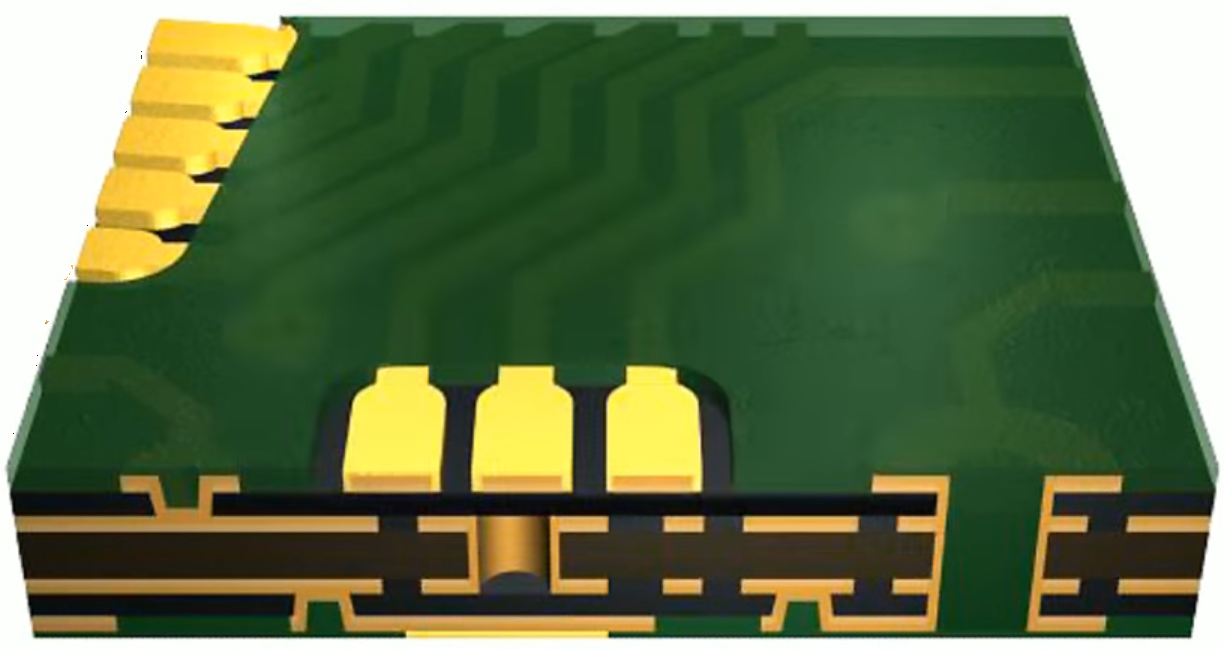
\includegraphics[scale=0.12]{obr20_Pokoveni.png}\\
			& Developing & & Metal plating
			\end{tabular}
		\end{center}
	\end{frame}
%------------------------------------------------------------------------------
	\begin{frame}
    \frametitle{Metal Plating}

		\begin{center}
			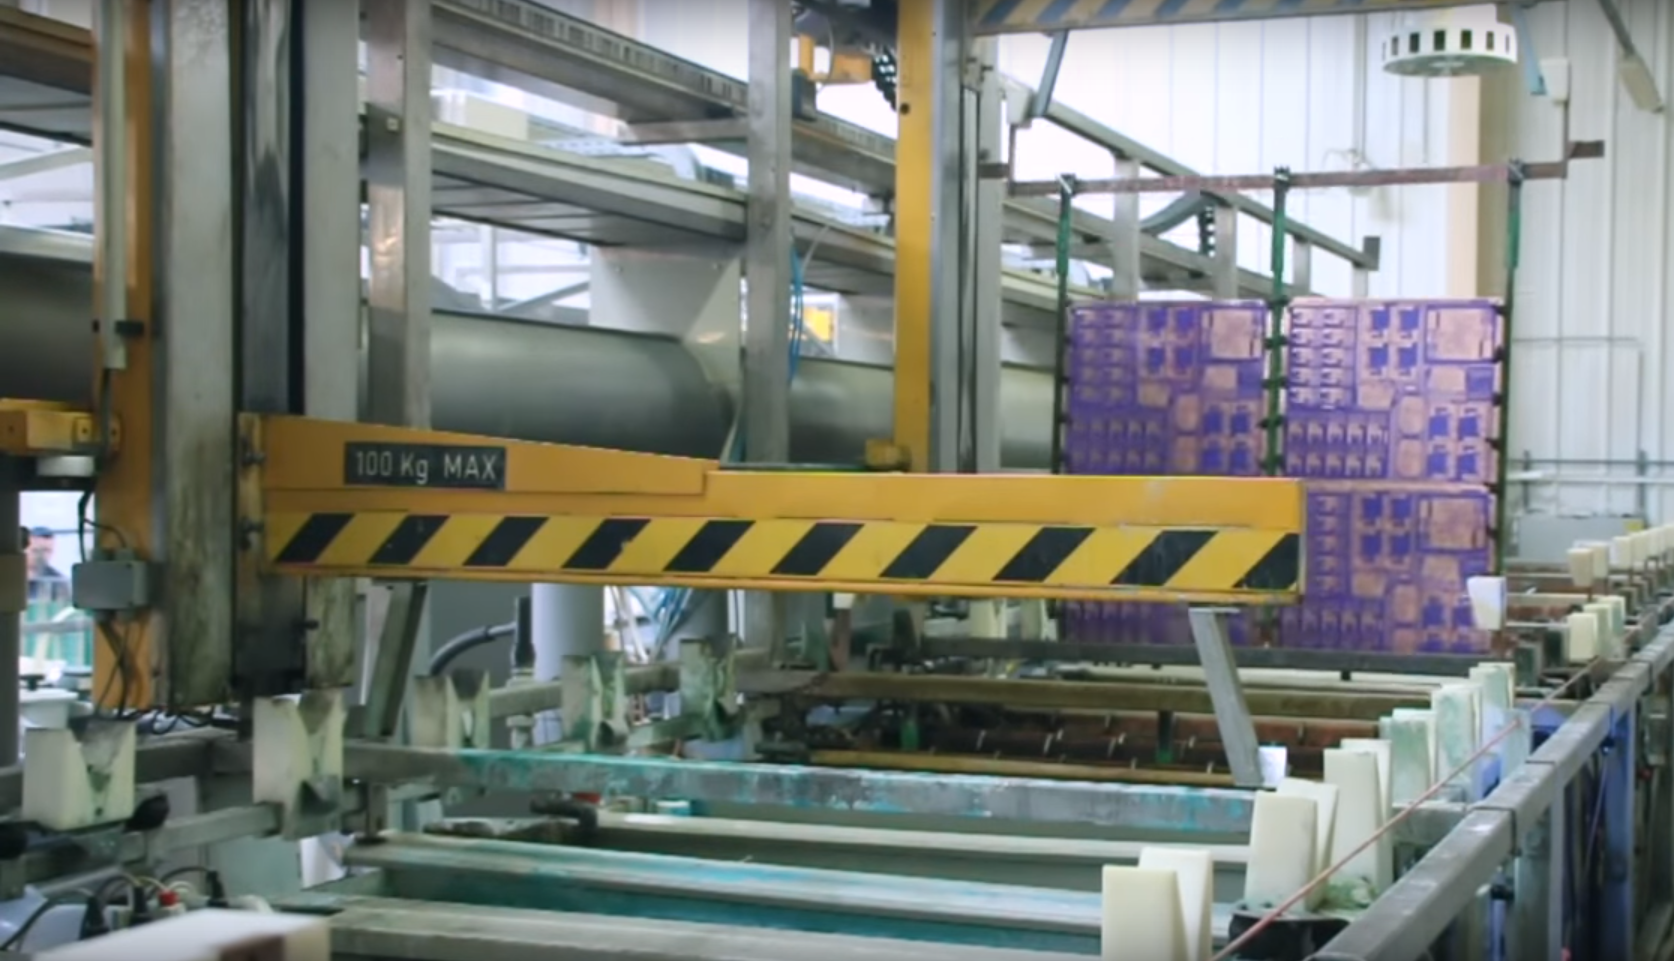
\includegraphics[scale=0.2]{obr22_procesProkovovani.png}
		\end{center}
		
	\end{frame}
%------------------------------------------------------------------------------
	\begin{frame}
    \frametitle{Resources}
	
		\begin{enumerate}
			\item http://www.isola-group.com/wp-content/uploads/
			\item https://www.youtube.com/watch?v=z4f-D1EKKD4
			\item https://www.youtube.com/watch?v=T7S40GYESbY
			\item https://www.youtube.com/watch?v=hpR4e1n0HKo\&t=204s
		\end{enumerate}
	\end{frame}
%------------------------------------------------------------------------------
\end{document}